%06chapterVergleich.tex

\chapter{Vorgehen}
\label{sec:Vorgehen}

Als Pascal die ganze Koordination übernahm, erstellte er anfangs ein Grobablauf \ref{fig:grobablauf}, der uns als Grundlage und gute Übersicht dienen sollte.

\begin{figure}[ht]
	\centering
	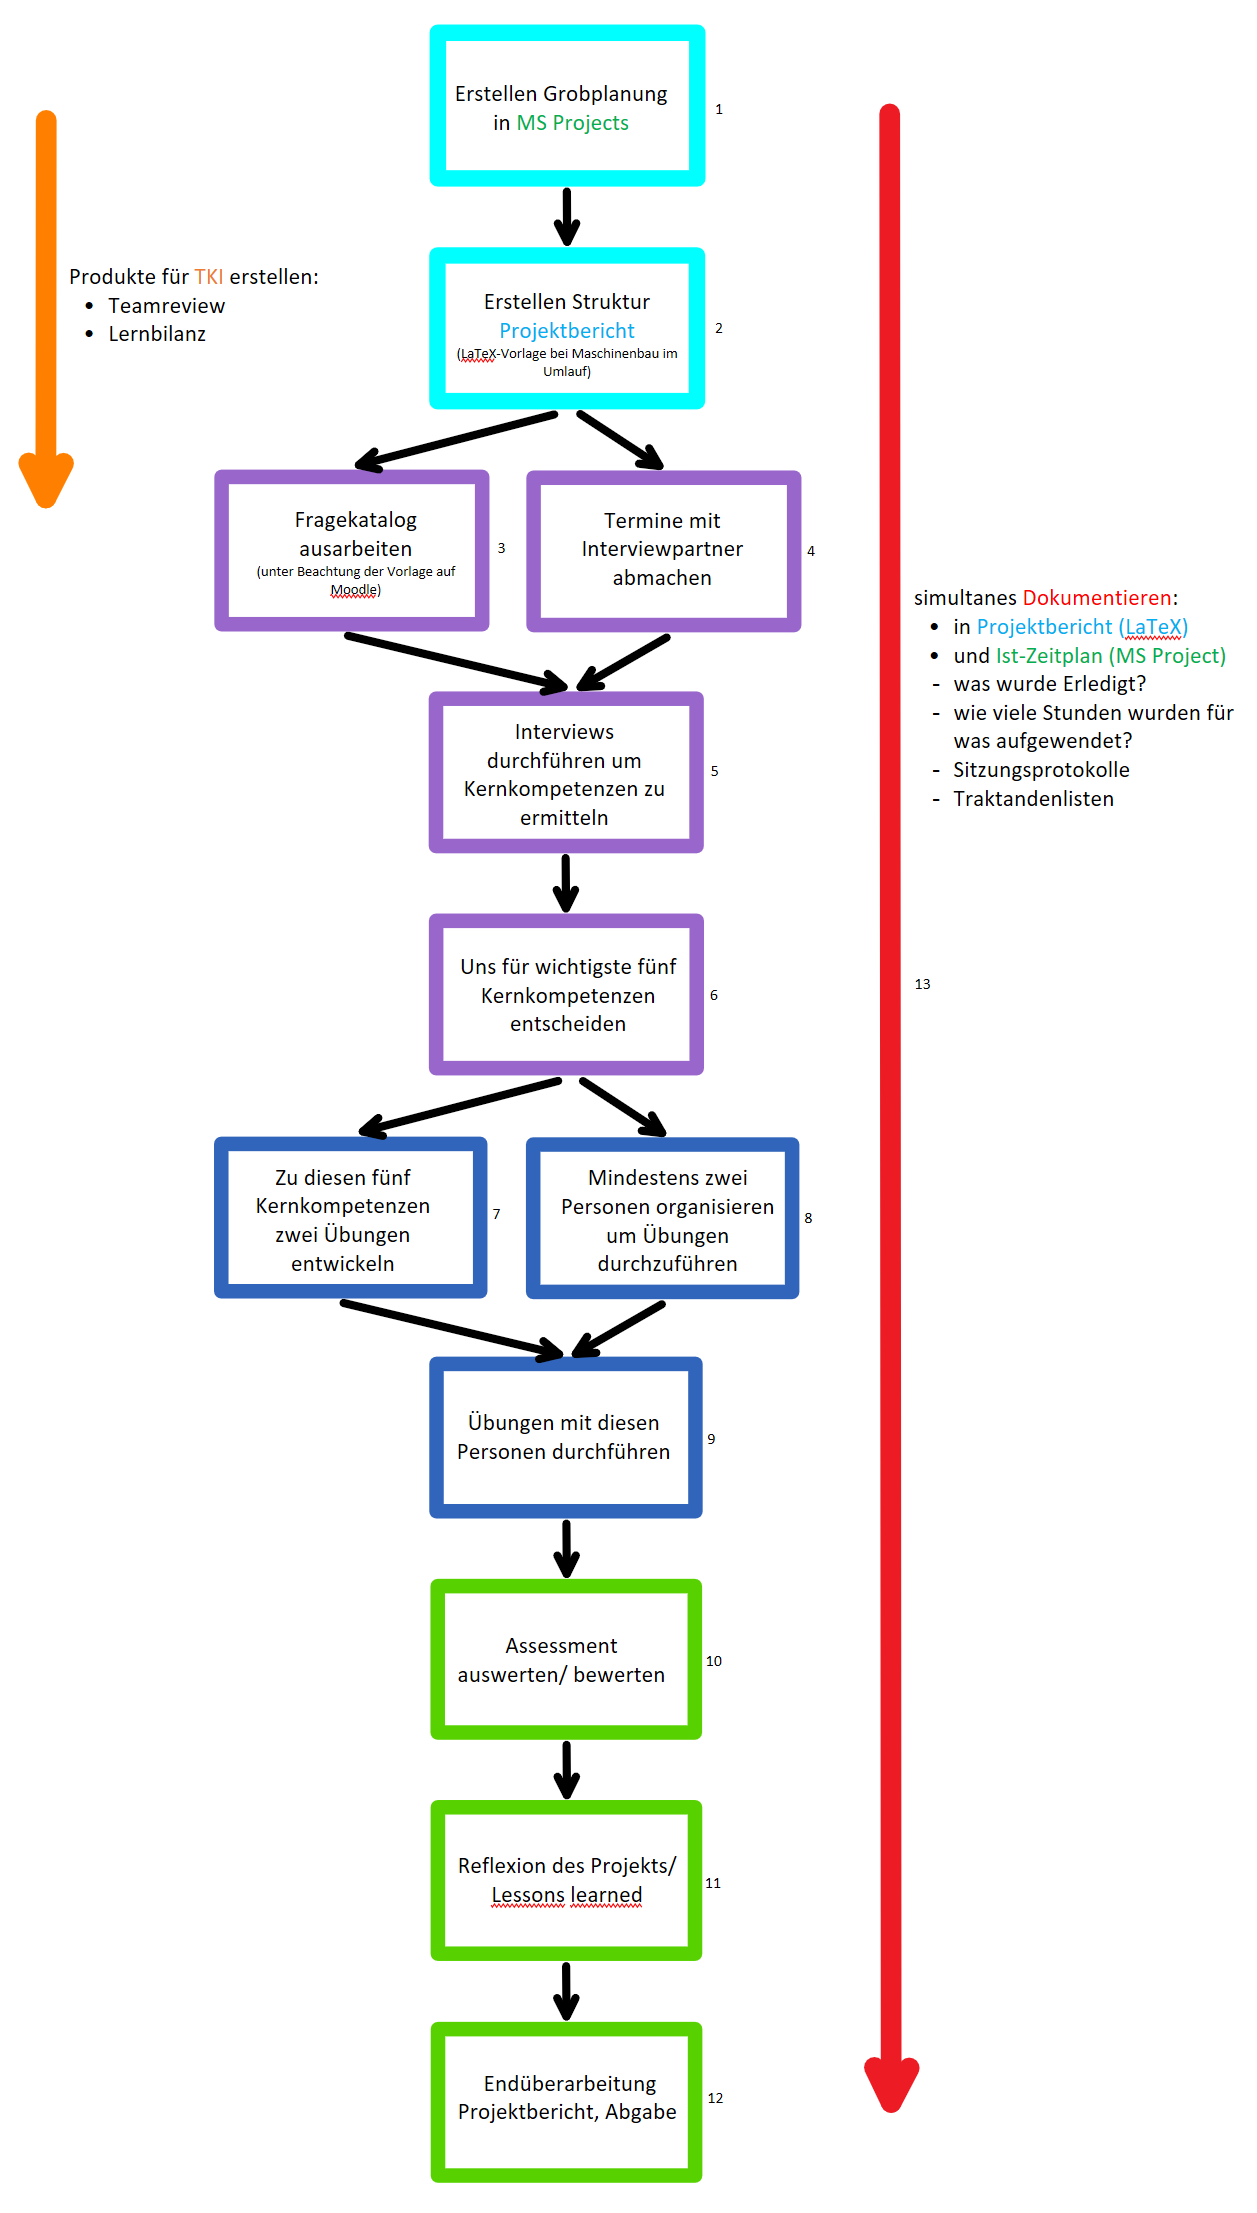
\includegraphics[width=0.9\textwidth]{images/Grobablauf.png}
	\caption{Grobablauf}
	\label{fig:grobablauf}
\end{figure}

Anschiessend hat er mittels MS Project eine Detailplanung \ref{fig:msproject} erstellt. Diese enthält alle Arbeiten inkl. Zeitvorgaben.

\begin{figure}[ht]
	\centering
	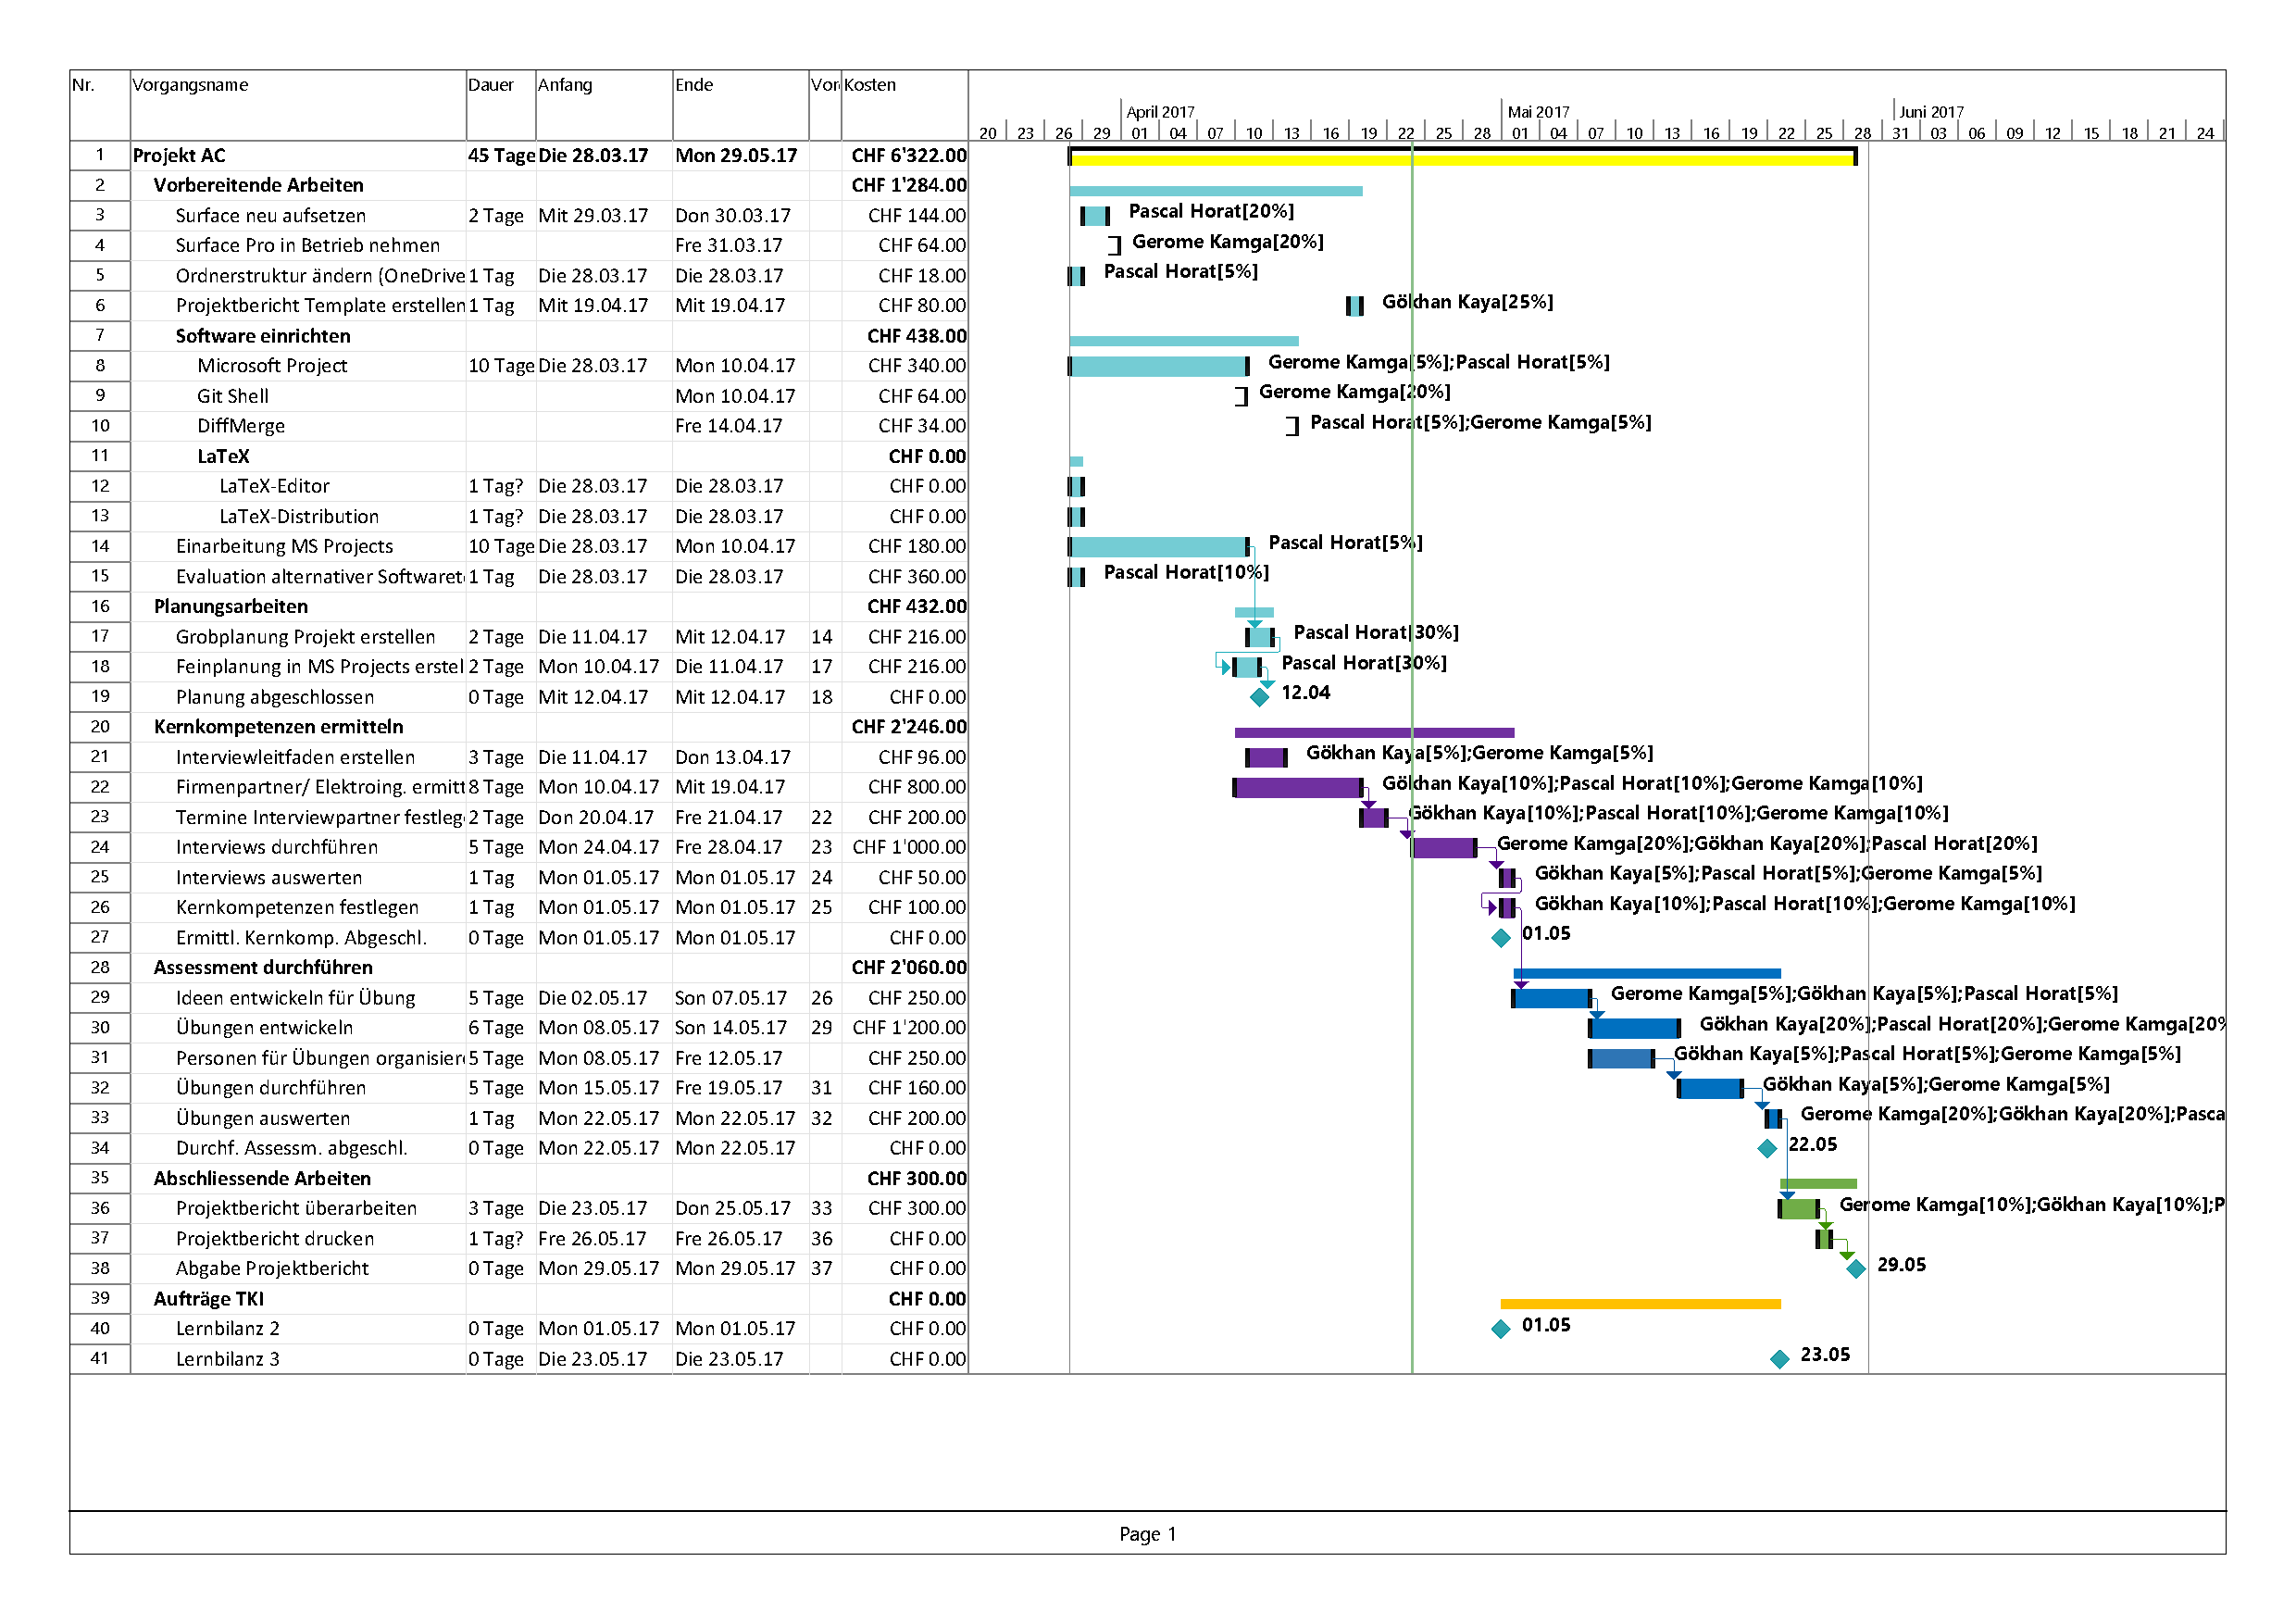
\includegraphics[width=1.7\textwidth, angle =270]{images/BaselineAC2.pdf}
	\caption{Baseline in MS Project}
	\label{fig:msproject}
\end{figure}

Um die Aufträge koordinieren zu können, hat Pascal schliesslich ein Excel-File erstellt und diese auf One-Drive geladen. Dieses File liess sich von allen (jedoch nicht Gleichzeitig) online bearbeiten und abspeichern. Pascal konnte nach den Fristen seine Kommentare dazu abgeben oder falls nötig dazu auffordern einige Korrekturen vorzunehmen. Je nach Stand der Arbeit wurden die Aufträge gemäss Bild \ref{fig:auftrage} farblich markiert. Gökhan und Gerome konnten jeweils eintragen, wie viel der Aufträge (in Prozente) bereits erledigt und wieviel Zeit dafür aufgewendet wurde. 

\begin{figure}[ht]
	\centering
	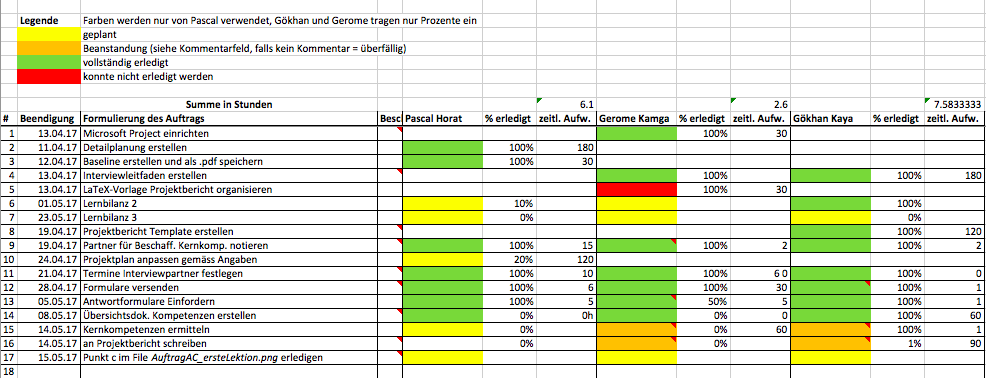
\includegraphics[width=1.1\textwidth]{images/Auftrage}
	\caption{Ausschnitt Auftragsaufteilung}
	\label{fig:auftrage}
\end{figure}

Da viele Arbeiten mittels dem Versionsverwaltungstool Git erledigt wurden, kann an dieser Stelle ebenfalls eine gute Übersicht über die tatsächlich erledigten Arbeiten gezeigt werden. Aufgrund der Grösse dieser Commit History ist sie im Anhang unter REFERENZ aufgeführt DIESER SATZ AUCH IN ANHANG --> Unten ist die Liste mit unseren tatsächlich hochgeladenen Änderungen inkl. unseren Kommentaren zu sehen.

%AB HIER KANN JEROME FORMATIEREN
%SteveGerome, Thu Jun 8 14:41:41 2017 +0200 : übersichtausschnitt Auftragsaufteilung 2 \\
%SteveGerome, Thu Jun 8 13:38:13 2017 +0200 : übersichtausschnitt Auftragsaufteilung 1 \\
%SteveGerome, Thu Jun 8 08:27:47 2017 +0200 : übersichtausschnitt Auftragsaufteilung \\
%kaya, Wed Jun 7 15:45:05 2017 +0200 : Bewertung fertiggestellt. Noch kommentieren \\
%Corumh, Wed Jun 7 14:35:31 2017 +0200 : Alles zusammen kompiliert \\
%kaya, Wed Jun 7 14:28:50 2017 +0200 : Merge branch 'master' of https://github.com/cruis1/tki Konflikt \\
%kaya, Wed Jun 7 14:28:35 2017 +0200 : Ein Teil der Bewertung geschrieben \\
%Corumh, Wed Jun 7 14:24:53 2017 +0200 : Auswertung Assessment weitergeschrieben \\
%Corumh, Wed Jun 7 12:00:57 2017 +0200 : Auswertung der Übung 2 weitergeschr. \\
%Corumh, Wed Jun 7 11:08:15 2017 +0200 : Auswertung des Assessments weitergeschr. \\
%Corumh, Wed Jun 7 10:49:07 2017 +0200 : Auswertung des Assessments angefangen \\
%Corumh, Wed Jun 7 09:37:18 2017 +0200 : Bewertungsanmerkungen Probanden angefangen \\
%Corumh, Wed Jun 7 09:15:48 2017 +0200 : Bewertungstabellen Probanden fertig \\
%Corumh, Tue Jun 6 19:47:35 2017 +0200 : Protokolle angepasst \\
%SteveGerome, Tue Jun 6 19:38:49 2017 +0200 : Sitzungsprotokolle verbessert 1 \\
%SteveGerome, Tue Jun 6 19:32:49 2017 +0200 : Sitzungsprotokolle verbesssert \\
%SteveGerome, Tue Jun 6 15:20:25 2017 +0200 : Commit History form. beendet \\
%Corumh, Tue Jun 6 15:06:20 2017 +0200 : Bewertung Probanden Selbstmanagement gem. \\
%Corumh, Tue Jun 6 13:28:31 2017 +0200 : Bewertung Probanden weitergeschr. \\
%Corumh, Tue Jun 6 13:05:02 2017 +0200 : Bewertung Probanden angefangen \\
%Corumh, Tue Jun 6 12:25:31 2017 +0200 : Einleitung angepasst \\
%Corumh, Tue Jun 6 12:20:58 2017 +0200 : gitignore angepasst \\
%Corumh, Tue Jun 6 12:16:57 2017 +0200 : gitignore angepasst \\
%Corumh, Tue Jun 6 12:14:32 2017 +0200 : gitignore angepasst \\
%Corumh, Tue Jun 6 11:58:05 2017 +0200 : Ablauf Assessment beschr. \\
%SteveGerome, Tue Jun 6 11:54:51 2017 +0200 : Commit History form. beendet \\
%SteveGerome, Tue Jun 6 11:34:53 2017 +0200 : Commit History form. weiter verbe. \\
%kaya, Tue Jun 6 11:25:39 2017 +0200 : Merge branch 'master' of https://github.com/cruis1/tki Merge \\
%kaya, Tue Jun 6 11:25:24 2017 +0200 : Mainfile Projektauftrag hinzugefügt \\
%Corumh, Tue Jun 6 11:22:24 2017 +0200 : Merge branch 'master' of https://github.com/cruis1/tki \\
%Corumh, Tue Jun 6 11:21:39 2017 +0200 : Commit History Formattierung verb. \\
%kaya, Tue Jun 6 11:21:37 2017 +0200 : Filevorlage Projektauftrag erstellt \\
%SteveGerome, Tue Jun 6 11:15:50 2017 +0200 : Commit History form. verb. \\
%SteveGerome, Tue Jun 6 11:09:43 2017 +0200 : trying \\
%SteveGerome, Tue Jun 6 11:08:57 2017 +0200 : trying \\
%SteveGerome, Tue Jun 6 11:05:35 2017 +0200 : trying \\
%SteveGerome, Tue Jun 6 11:02:12 2017 +0200 : trying \\
%Corumh, Tue Jun 6 10:54:42 2017 +0200 : gitignore Assessment erstellt \\
%kaya, Tue Jun 6 10:30:00 2017 +0200 : Commit history hinzugefügt \\
%kaya, Thu Jun 1 16:15:20 2017 +0200 : Diverse Änderungen im Abschnit Teamgrundlagen und Vorgehen \\
%kaya, Thu Jun 1 15:32:12 2017 +0200 : Merge branch 'master' of https://github.com \\
%kaya, Thu Jun 1 16:15:20 2017 +0200 : Diverse Änderungen im Abschnitt Teamgrundlagen und Vorgehen \\
%kaya, Thu Jun 1 15:32:12 2017 +0200 : Merge branch 'master' of https://github.com/cruis1/tki merge \\
%kaya, Thu Jun 1 15:32:03 2017 +0200 : Teil Vorgehen überarbeitet \\
%Corumh, Thu Jun 1 15:25:52 2017 +0200 : Übung Selbstmanag. mitzut. Infos fertigg. \\
%kaya, Thu Jun 1 14:44:34 2017 +0200 : Merge branch 'master' of https://github.com/cruis1/tki böö \\
%kaya, Thu Jun 1 14:44:23 2017 +0200 : Teil Vorgehen geschrieben \\
%Corumh, Thu Jun 1 14:42:44 2017 +0200 : Übung Selbstmanag. mitzut. Infos angef. \\
%Corumh, Thu Jun 1 13:58:12 2017 +0200 : Übung Selbstmanag. verfeinert \\
%Corumh, Thu Jun 1 13:19:40 2017 +0200 : Merge branch 'master' of https://github.com/cruis1/tki \\
%Corumh, Wed May 31 17:51:22 2017 +0200 : Übung Selbstmanag. alle Aufgabe fertig \\
%kaya, Wed May 31 16:02:27 2017 +0200 : Teil Klärung der Aufgabenstellung angefangen \\
%kaya, Wed May 31 15:31:15 2017 +0200 : Merge branch 'master' of https://github.com/cruis1/tki kei ahnig was lauft \\
%kaya, Wed May 31 15:28:27 2017 +0200 : Fragetext korrigiert \\
%Corumh, Wed May 31 15:22:57 2017 +0200 : Merge branch 'master' of https://github.com/cruis1/tki \\
%Corumh, Wed May 31 15:22:32 2017 +0200 : Übung Selbstmanag. E-Mail-Aufgabe fertig \\
%kaya, Wed May 31 15:12:52 2017 +0200 : Einleitung korrigiert \\
%kaya, Wed May 31 14:46:12 2017 +0200 : Kapitel Teamgrundlagen geschrieben. Achtung: Kann fehler verursachen beim kompilieren \\
%kaya, Wed May 31 12:17:54 2017 +0200 : Vorbereitungen für Teamvertrag img ordner hinzugefügt \\
%Corumh, Wed May 31 12:16:43 2017 +0200 : Übung Selbstmanag. Kreuzwortraetsel fertig \\
%kaya, Wed May 31 11:51:52 2017 +0200 : Erster Teil der Einleitung \\
%Corumh, Wed May 31 11:48:57 2017 +0200 : Übung Selbstmanag. Messbericht fast fertig \\
%kaya, Wed May 31 10:56:55 2017 +0200 : kleine korrekturen \\
%Corumh, Wed May 31 10:49:15 2017 +0200 : Übung Selbstmanag. Messbericht weitergeschr. \\
%kaya, Wed May 31 10:40:43 2017 +0200 : Merge branch 'master' of https://github.com/cruis1/tki testmerge \\
%kaya, Wed May 31 10:40:15 2017 +0200 : Tabelle korrigiert \\
%Corumh, Wed May 31 10:39:52 2017 +0200 : Übung Selbstmanag. Messbericht angef. \\
%Kaya, Tue May 30 20:30:33 2017 +0200 : Diverse Tabellen hinzugefügt \\
%Kaya, Tue May 30 19:56:43 2017 +0200 : Viele Korrekturen und weitere Arbeiten \\
%kaya, Tue May 30 18:11:52 2017 +0200 : Teil Test1 hinzugefügt \\
%Corumh, Tue May 30 16:27:24 2017 +0200 : Übung Selbstmanag. Bewertungskriterien weiter beschr. \\
%Corumh, Tue May 30 15:19:04 2017 +0200 : Beobachtungsinstr. Selbstmanag. Bewertungskriterien beschr. \\
%kaya, Tue May 30 14:47:56 2017 +0200 : nüt \\
%Corumh, Tue May 30 14:29:34 2017 +0200 : Beobachtungsinstr. Selbstmanag. Bewertung \\
%Corumh, Tue May 30 13:53:05 2017 +0200 : Beobachtungsinstr. Selbstmanag. Aufgaben weiter beschrieben \\
%Corumh, Mon May 29 17:14:46 2017 +0200 : Beobachtungsinstr. Selbstmanag. Aufgaben beschrieben \\
%Corumh, Mon May 29 16:10:04 2017 +0200 : Beobachtungsinstr. Selbstmanag. Detail beschrieben \\
%Corumh, Mon May 29 16:06:30 2017 +0200 : Beobachtungsinstr. Selbstmanag. weiter beschrieben \\
%Corumh, Mon May 29 15:56:12 2017 +0200 : Beobachtungsinstr. Selbstmanag. beschrieben \\
%Kaya, Thu May 25 20:42:47 2017 +0200 : Korrekturen und weitere Arbeiten \\
%Corumh, Sun May 14 16:07:20 2017 +0200 : Projektbericht Fehler behoben \\
%kaya, Mon May 8 16:01:52 2017 +0200 : readme update \\
%kaya, Mon May 8 16:00:37 2017 +0200 : readme update \\
%kaya, Mon May 8 15:52:42 2017 +0200 : korrekturen \\
%kaya, Mon May 8 15:40:18 2017 +0200 : Kernkompetenz Auswertung hinzugefügt, Assessmentbericht Interviewteil weitergeschrieben \\
%kaya, Mon May 8 14:59:29 2017 +0200 : HILFE file überarbeitet \\
%kaya, Mon May 8 14:58:12 2017 +0200 : HILFE file erstellt für die hartnäckige merge konflikt \\
%Corumh, Mon Apr 24 16:35:48 2017 +0200 : Projektbericht Referenz Website \\
%kaya, Mon Apr 24 16:31:32 2017 +0200 : ksjdksj \\
%Corumh, Mon Apr 24 16:26:53 2017 +0200 : Projektbericht Referenz Website \\
%Corumh, Mon Apr 24 16:26:05 2017 +0200 : Projektbericht Referenz Website \\
%kaya, Mon Apr 24 16:21:51 2017 +0200 : nüt spannends \\
%kaya, Mon Apr 24 15:11:00 2017 +0200 : Ordner Projektbericht gelöscht \\
%kaya, Mon Apr 24 12:12:08 2017 +0200 : Fragekatalog verbessert 2 \\
%kaya, Mon Apr 24 12:05:55 2017 +0200 : Fragenkatalog korrigiert \\
%kaya, Wed Apr 19 19:09:19 2017 +0200 : Assessmentbericht template fertig \\
%kaya, Wed Apr 19 15:34:54 2017 +0200 : Fragekatalog nachgebessert \\
%kaya, Wed Apr 12 21:02:19 2017 +0200 : Fragenkatalog angepasst \\
%Corumh, Mon Apr 3 23:26:16 2017 +0200 : TR3 Orthografie korrigiert \\
%Corumh, Mon Apr 3 23:02:35 2017 +0200 : TR3 komplett überarbeitet \\
%Corumh, Mon Apr 3 20:29:41 2017 +0200 : TR3 Protokoll eingefügt \\
%kaya, Mon Apr 3 20:00:33 2017 +0200 : TR3 fast fertig \\
%kaya, Mon Apr 3 18:45:59 2017 +0200 : Gruppeneinschätzung fertig \\
%kaya, Mon Apr 3 16:48:33 2017 +0200 : TR3 continue \\
%Corumh, Mon Apr 3 16:01:09 2017 +0200 : TR3 Web-Pic eingefügt \\
%Corumh, Mon Apr 3 15:57:15 2017 +0200 : Merge branch 'master' of https://github.com/cruis1/tki \\
%kaya, Mon Apr 3 15:56:59 2017 +0200 : Arbeit... \\
%Corumh, Mon Apr 3 14:52:12 2017 +0200 : TR2 Änderig\\
%Corumh, Mon Apr 3 14:08:39 2017 +0200 : TR3 Vorlage pagebreak entfernt\\
%kaya, Mon Apr 3 14:04:13 2017 +0200 : TR3 vorlage angepasst\\
%Corumh, Mon Apr 3 02:27:49 2017 +0200 : TR3 Vorlage Fehler entfernt\\
%kaya, Mon Mar 27 16:41:16 2017 +0200 : nichts nennenswertes\\
%Corumh, Mon Mar 27 15:50:50 2017 +0200 : TR3 Vorlage angefangen\\
%Corumh, Mon Mar 27 12:11:55 2017 +0200 : TR2 in finale Form gebracht\\
%kaya, Mon Mar 27 11:08:49 2017 +0200 : pagebreak aenderungen auskommentiert\\
%Corumh, Mon Mar 27 01:59:09 2017 +0200 : TR2 zusätzliche Literatur eingefügt\\
%Corumh, Mon Mar 27 00:38:32 2017 +0200 : TR2 kompl. überarb. (Rechtschreibef.) und erweitert\\
%Corumh, Sun Mar 26 17:45:31 2017 +0200 : TR2 fast fertig\\
%Corumh, Sun Mar 26 15:27:03 2017 +0200 : an TR2 weitergearbeitet\\
%SteveGerome, Sun Mar 26 15:16:44 2017 +0200 : weitergeschrieben TR2\\
%Corumh, Sun Mar 26 14:55:44 2017 +0200 : an TR2 weitergearbeitet, Bilder eingefügt\\
%Corumh, Thu Mar 23 14:24:16 2017 +0100 : an TR2 weitergearbeitet, Bilder eingefügt\\
%Corumh, Thu Mar 23 14:03:00 2017 +0100 : .rtf gelöscht\\
%Corumh, Thu Mar 23 13:59:07 2017 +0100 : .log gelöscht\\
%Corumh, Thu Mar 23 13:57:40 2017 +0100 : TR2 Formattierung verschönert und weitergeschrieben\\
%Corumh, Thu Mar 23 13:16:42 2017 +0100 : TR2 weitergearbeitet\\
%SteveGerome, Wed Mar 22 21:23:31 2017 +0100 : zweiter Commit :-)\\
%Corumh, Wed Mar 22 21:18:40 2017 +0100 : einige Korrekturen in TR2\\
%SteveGerome, Wed Mar 22 21:15:22 2017 +0100 : erster Commit :-)\\
%Corumh, Wed Mar 22 20:27:56 2017 +0100 : neueste Teamreview 2 Version Upload\\
%kaya, Wed Mar 22 20:22:35 2017 +0100 : shit happened\\
%kaya, Wed Mar 22 20:15:19 2017 +0100 : Selbsteinschätzung bearbeitet\\
%Corumh, Wed Mar 22 20:10:43 2017 +0100 : hoffentlich klappts\\
%kaya, Wed Mar 22 20:06:50 2017 +0100 : Merge branch 'master' of https://github.com/cruis1/tki\\
%kaya, Wed Mar 22 20:06:26 2017 +0100 : Selbsteinschätzung überarbeitet\\
%Corumh, Wed Mar 22 20:05:09 2017 +0100 : hoffentlich klappts\\
%kaya, Wed Mar 22 19:45:55 2017 +0100 : Merge branch 'master' of https://github.com/cruis1/tki\\
%kaya, Wed Mar 22 19:44:30 2017 +0100 : Fremdeinschätzung grob ferig\\
%Corumh, Wed Mar 22 19:34:07 2017 +0100 : zum Abgliche\\
%Corumh, Wed Mar 22 19:02:33 2017 +0100 : resolve merge error\\
%Corumh, Wed Mar 22 18:45:58 2017 +0100 : Teamreview 2 Selbsteinsch. bearb\\
%kaya, Wed Mar 22 18:45:31 2017 +0100 : test\\
%kaya, Wed Mar 22 18:38:25 2017 +0100 : Merge branch 'master' of https://github.com/cruis1/tki\\
%kaya, Wed Mar 22 18:34:32 2017 +0100 : removed Fremdeinschätzung\\
%Corumh, Wed Mar 22 18:32:15 2017 +0100 : Teamreview 2 Selbsteinsch. bearb\\
%kaya, Wed Mar 22 18:23:28 2017 +0100 : selbsteinschätzung erstellt\\
%kaya, Wed Mar 22 17:04:09 2017 +0100 : selbsteinschätzung erstellt\\
%Corumh, Tue Mar 21 17:35:53 2017 +0100 : Teamreview 2 weitererstellt, Referenzen funktionieren\\
%Corumh, Tue Mar 21 17:32:52 2017 +0100 : Teamreview 2 weitererstellt, Referenzen funktionieren\\
%Corumh, Tue Mar 21 13:56:24 2017 +0100 : Teamreview 2 Struktur erstellt, Referenzen funktionieren\\
%Corumh, Tue Mar 21 12:09:38 2017 +0100 : Teamreview 2 Template angefangen\\
%Corumh, Tue Mar 21 11:30:41 2017 +0100 : Ordnerstruktur geändert und noch mehr aufgeräumt\\
%Corumh, Tue Mar 21 11:18:35 2017 +0100 : Ordnerstruktur geändert und aufgeräumt\\
%Corumh, Tue Mar 21 11:10:12 2017 +0100 : Upload TR2\\
%Corumh, Mon Mar 20 20:12:37 2017 +0100 : Penis\\
%Corumh, Mon Mar 20 19:28:05 2017 +0100 : Upload TR2\\
%Corumh, Mon Mar 20 16:13:56 2017 +0100 : Upload TR2\\
%Corumh, Mon Mar 20 15:07:02 2017 +0100 : Upload TR2\\
%Corumh, Mon Mar 20 13:58:25 2017 +0100 : Upload Vorlage TR2\\
%Corumh, Mon Mar 20 12:29:35 2017 +0100 : Reflexion Sitzung finalisiert\\
%Corumh, Fri Mar 17 17:07:49 2017 +0100 : Reflexion Sitzung erstellt\\
%Corumh, Fri Mar 17 16:22:08 2017 +0100 : Traktl. final.\\
%Corumh, Thu Mar 16 20:41:02 2017 +0100 : Upload Traktl. akt.\\
%Corumh, Thu Mar 16 20:10:54 2017 +0100 : Upload Traktl.\\
%Corumh, Thu Mar 16 19:40:46 2017 +0100 : Konflikt bereinige\\
%Corumh, Mon Mar 13 20:53:49 2017 +0100 : Reflexion TR1 erstellt\\
%kaya, Mon Mar 13 17:19:59 2017 +0100 : Merge branch 'master' of https://github.com/cruis1/tki\\
%kaya, Mon Mar 13 17:06:10 2017 +0100 : Name angepasst\\
%kaya, Mon Mar 13 17:04:04 2017 +0100 : Name angepasst\\
%kaya, Mon Mar 13 17:02:42 2017 +0100 : Name angepasst\\
%Corumh, Mon Mar 13 16:46:47 2017 +0100 : Reflexion TR1 erstellt\\
%kaya, Mon Mar 13 16:32:36 2017 +0100 : Änderungen an trakdandenliste\\
%kaya, Mon Mar 13 16:13:56 2017 +0100 : Trakdandenliste explizit vervollständigt\\
%kaya, Mon Mar 13 15:42:03 2017 +0100 : Fragenkatalog fertiggestellt\\
%kaya, Mon Mar 13 15:10:35 2017 +0100 : Fragenkatalog Vorlage erstellt\\
%kaya, Mon Mar 13 14:31:25 2017 +0100 : Fragenkatalog erstellt\\
%Corumh, Mon Mar 13 12:35:32 2017 +0100 : Merge branch 'master' of https://github.com/cruis1/tki\\
%Corumh, Mon Mar 13 12:34:18 2017 +0100 : Regeldokument finalisiert\\
%Columh, Sun Mar 12 23:49:13 2017 +0100 : Add files via upload\\
%kaya, Sun Mar 12 20:20:00 2017 +0100 : trakdandenliste\_vorlage grob fertig\\
%kaya, Sun Mar 12 18:50:06 2017 +0100 : trakdandenliste erstellt\\
%Corumh, Thu Mar 9 17:49:18 2017 +0100 : Regeldokument erweitert mit Bildern\\
%Corumh, Thu Mar 9 10:47:33 2017 +0100 : Regeldokument erweitert\\
%Corumh, Tue Mar 7 13:54:55 2017 +0100 : Regeldokument erstellt\\
%kaya, Mon Mar 6 16:56:25 2017 +0100 : Aufträge aktualisiert\\
%kaya, Mon Mar 6 16:29:39 2017 +0100 : teamreview update\\
%kaya, Mon Mar 6 15:29:30 2017 +0100 : teamreview bearbeitet\\
%kaya, Mon Mar 6 14:55:55 2017 +0100 : Ordner umbenannt und teamreview erstellt\\
%Corumh, Mon Mar 6 14:07:14 2017 +0100 : LaTex Template verbessert\\
%Corumh, Mon Mar 6 14:01:18 2017 +0100 : LaTex Template erstellt\\
%Corumh, Mon Mar 6 12:02:56 2017 +0100 : LaTex Template angefangen\\
%Corumh, Sun Mar 5 20:23:42 2017 +0100 : ToDo angepasst\\
%cruis1, Sun Mar 5 00:18:42 2017 +0100 : Delete\_config.yml\\
%kaya, Sun Mar 5 00:14:02 2017 +0100 : Merge branch 'master' of https://github.com/cruis1/tki\\
%cruis1, Sun Mar 5 00:10:44 2017 +0100 : Delete\_config.yml\\
%kaya, Sun Mar 5 00:04:13 2017 +0100 : doodle zu moodle geändert :)\\
%cruis1, Sun Mar 5 00:01:11 2017 +0100 : Set theme jekyll-theme-cayman\\
%kaya, Sat Mar 4 23:52:00 2017 +0100 : Alle files synchronisiert md file update\\
%kaya, Sat Mar 4 23:36:00 2017 +0100 : Links hinzugefügt\\
%cruis1, Sat Mar 4 23:31:16 2017 +0100 : Delete new.md\\
%kaya, Sat Mar 4 23:09:51 2017 +0100 : edit readme and add new.md s\\
%cruis1, Sat Mar 4 22:15:50 2017 +0100 : Initial commit\\
%%BIS HIER
%
%%BEFEHL: git log --pretty=format:"%an, %ar : %s"
%%BEFEHL evt. besser: git log --pretty=format:"%an, %ad : %s"
%%https://git-scm.com/book/tr/v2/Git-Basics-Viewing-the-Commit-History
